\subsection{Definition of Terms}
\begin{frame}
\frametitle\insertsection
	\framesubtitle\insertsubsection
	\vspace{-2em}
	\begin{itemize}
		\item {\textbf{Tracking} is the processing of measurements obtained from a target in order to maintain an estimate of its current state.}
		\item {\textbf{Measurements} are noise-corrupted	observations related to the state of a target.}
		\item {The \textbf{state} is the set of measured and estimated target parameters.}
		\item {A \textbf{track} is a state trajectory estimated from a set of measurements that are believed to be from the same target.}
	\end{itemize}
\end{frame}
\begin{frame}
	\frametitle\insertsection
	\framesubtitle\insertsubsection
	\vspace{-2em}
	Multi Target Tracking aims to:
	\begin{itemize}
		\item {acquire all of data as it is produced by the sensor.}
		\item {identify how many objects there are}
		\item {obtain estimates of the state vectors (position, velocity, etc.) of each object.}
	\end{itemize}
\end{frame}
\subsection{Multi Target Tracking Problems}
\begin{frame}
	\frametitle\insertsection
	\framesubtitle\insertsubsection
	\vspace{-2em}
	\textbf{Difficulties of Multi Target Tracking}
	\vspace{1em}
	\begin{itemize}
		\item {A target's position is only observed (measured) at discrete points in time.}
		\item {The measurements are noisy.}
		\item {There are measurements that are not from any target.}
		\item {The correct measurement is not always used.}
		\item {The intent of the target is not known.}
	\end{itemize}
\end{frame}
\begin{frame}
	\frametitle\insertsection
	\framesubtitle\insertsubsection
	\vspace{-2em}
	\begin{figure}
		\caption{\textbf{Multi Target Tracking Problem -- Example}}
		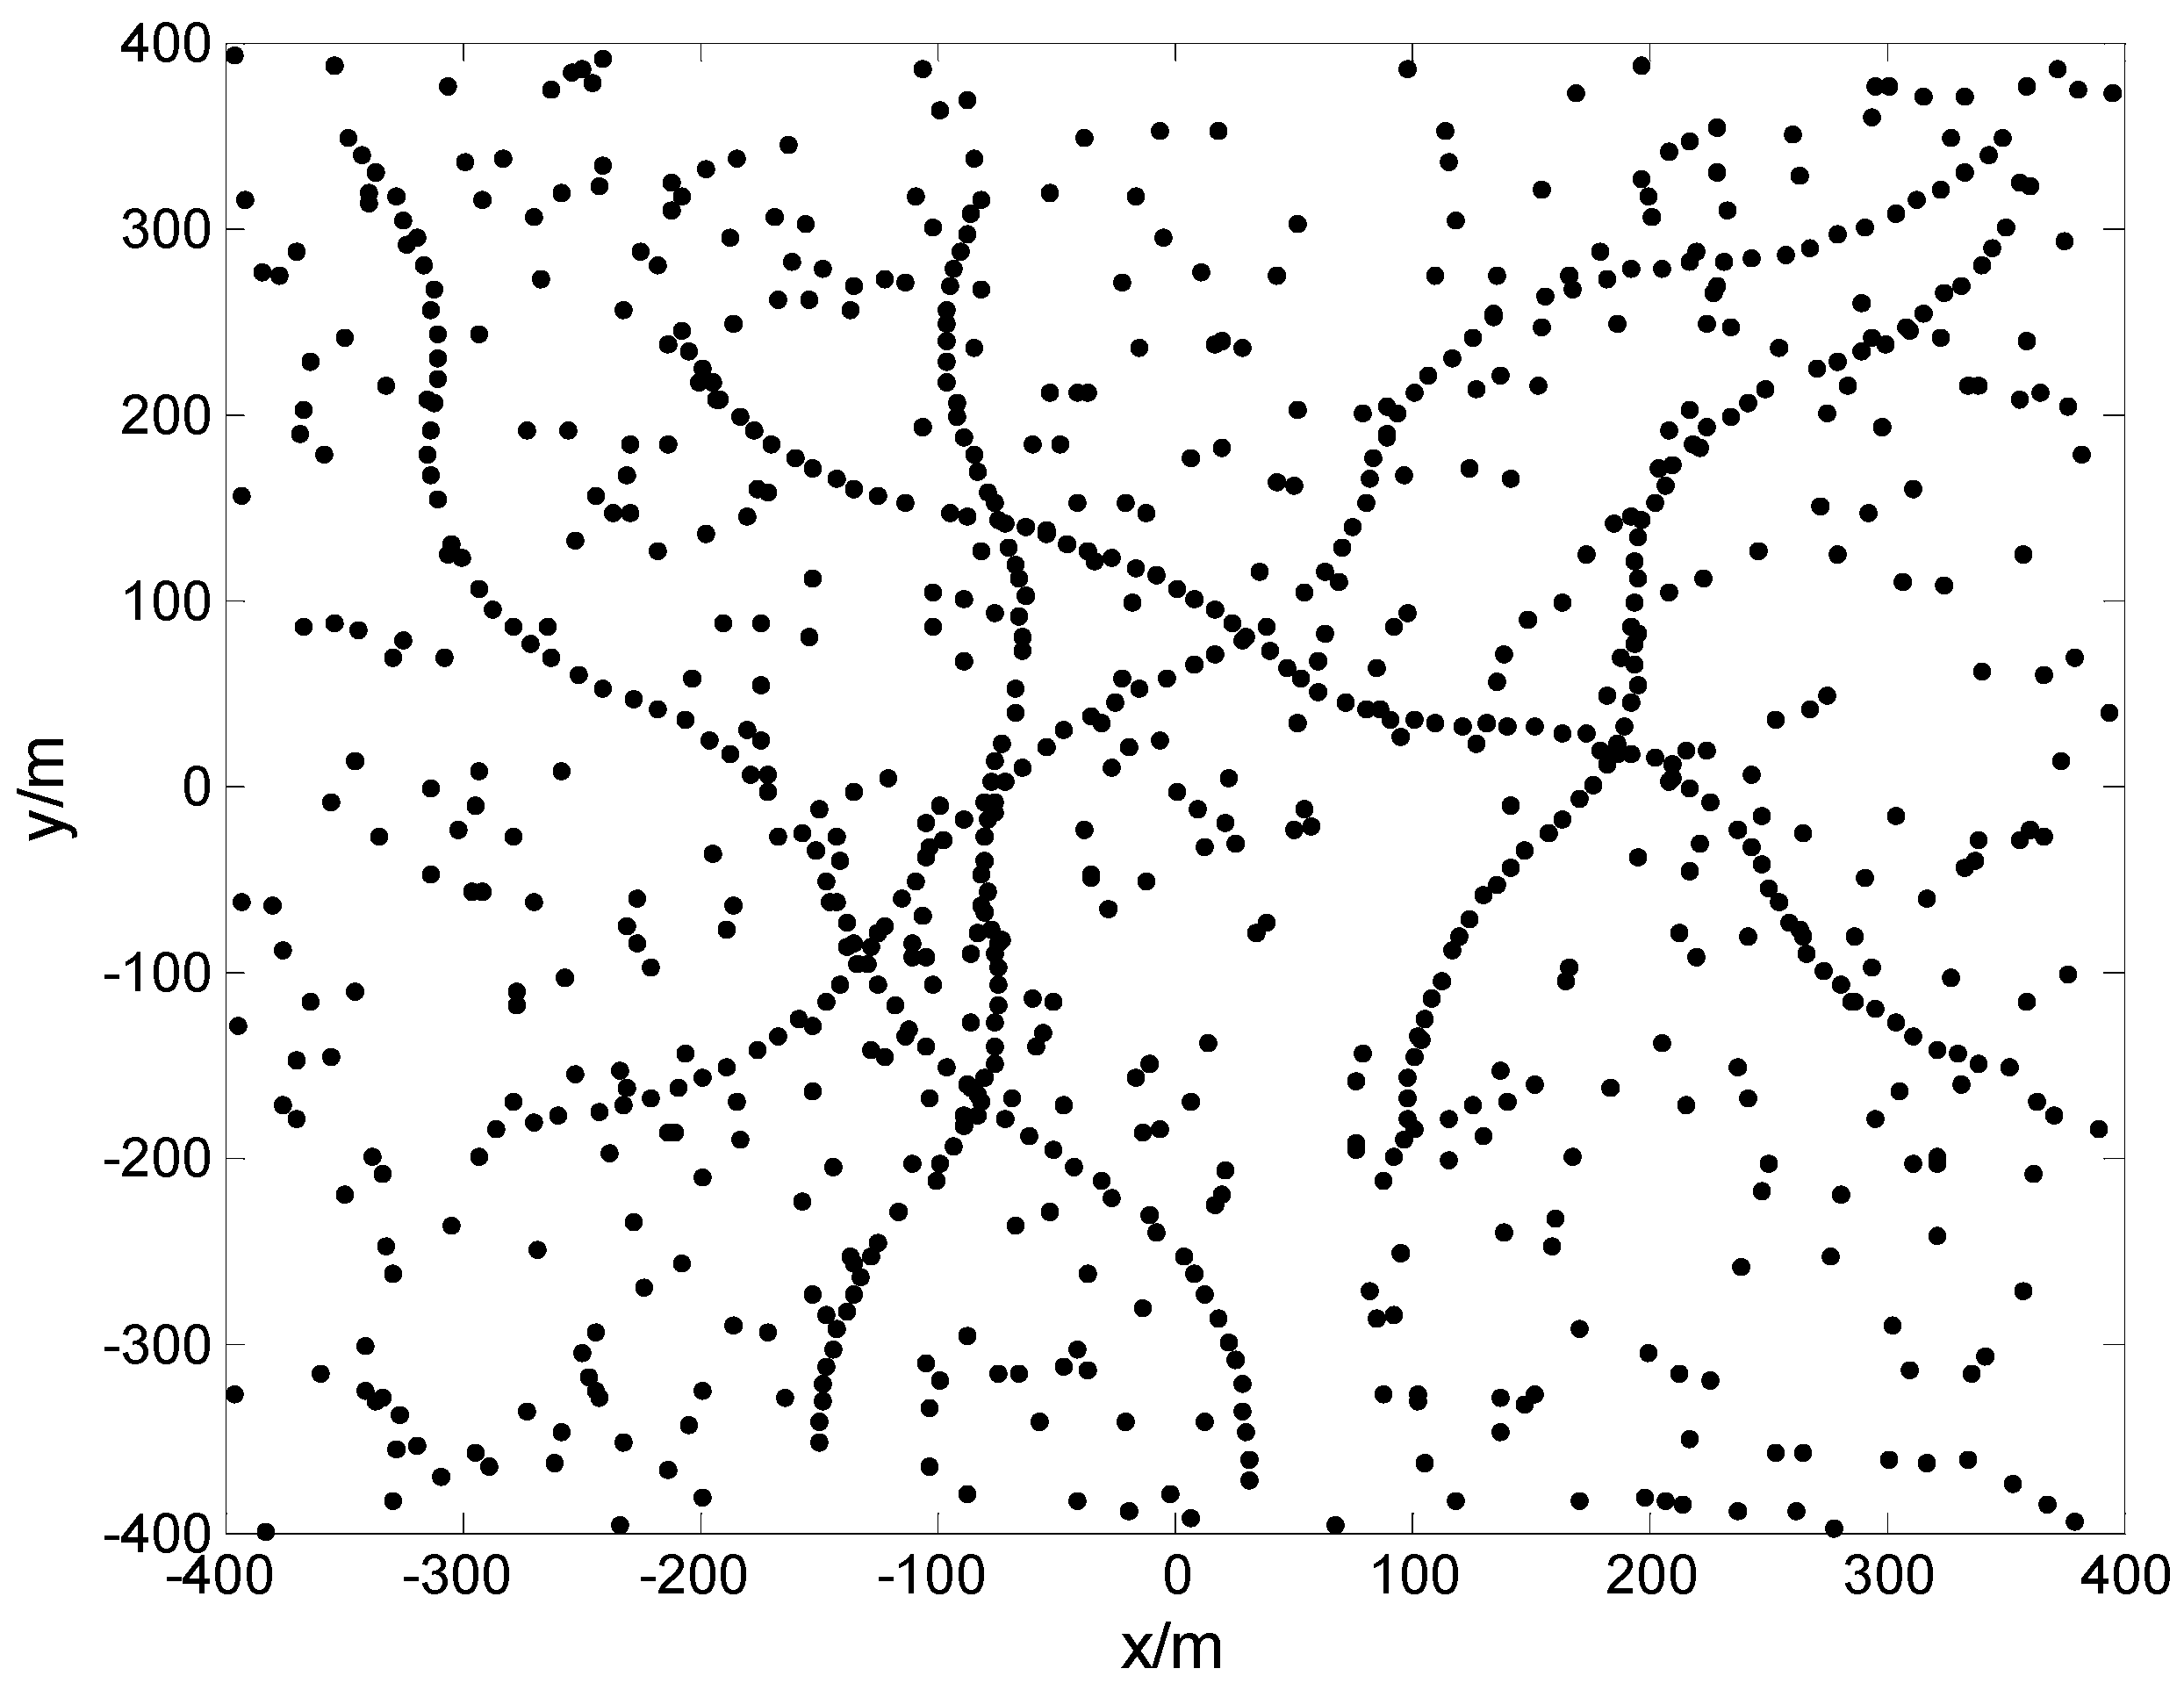
\includegraphics[scale=0.75]{./img/mtt-problems}
	\end{figure}
\end{frame}
\subsection{Tracking Function}
\begin{frame}
	\frametitle\insertsection
	\framesubtitle\insertsubsection
	\vspace{-1em}
	\begin{itemize}
		\item {Correlation}
		\item {Association}
		\item {State Estimation}
		\item {Track Initiation \& Management}
	\end{itemize}
\end{frame}
\begin{frame}
	\frametitle\insertsection
	\framesubtitle\insertsubsection
	\vspace{-2em}
	\begin{figure}
		\caption{\textbf{Functional Diagram -- Tracking System}}
		\scalebox{1}{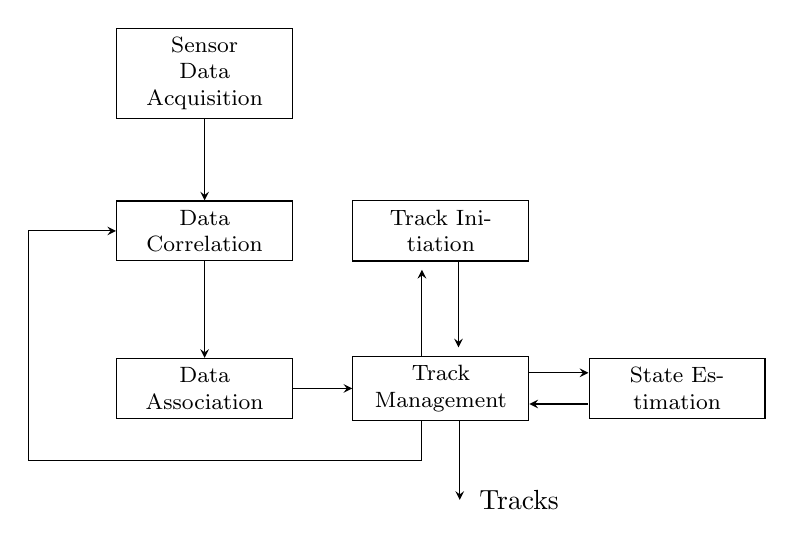
\begin{tikzpicture}[xscale=1,yscale=1,
	square/.style={rectangle, draw=black, text width=20mm, align=center, font=\footnotesize},
	label/.style={text width=5mm, align=center},
	node distance= 2cm, >=stealth]
	
	%Nodes
	\node[square]	(sda)	at (0,0) {Sensor\\Data\\Acquisition};
	\node[square]	(dc)	[below of=sda] {Data\\Correlation};
	\node[square]	(da)	[below of=dc] {Data\\Association};
	\node[square, xshift=1cm]	(ti)	[right of=dc] {Track Initiation};
	\node[square]	(tm)	[below of=ti] {Track\\Management};
	\node[square, xshift=1cm]	(se)	[right of=tm] {State Estimation};
	
	%Lines
	\draw[black, ->] (sda) -- (dc);
	\draw[black, ->] (dc) -- (da);
	\draw[black, ->] (da) -- (tm);
	\draw[black, ->] (ti.300) -- ++(0,-1.09);
	\draw[black, ->] (tm.120) -- ++(0,1.09);
	\draw[black, ->] (tm.10) -- ++(0.75,0);
	\draw[black, <-] (tm.350) -- ++(0.75,0);
	\draw[black, ->] (tm.240) -- ++(0,-0.5) -- ++(-5,0) |- (dc.west);
	\draw[black, ->] (tm.300) -- ++(0,-1) node[label, xshift=5mm] {Tracks};
\end{tikzpicture}}
	\end{figure}
\end{frame}
\begin{frame}
	\frametitle\insertsection
	\framesubtitle\insertsubsection
	\vspace{-2em}
	\begin{figure}
		\caption {\textbf{Tracking Process}}
		\scalebox{1}{\begin{tikzpicture}[xscale=1,yscale=1,
	round/.style={circle, inner sep=0pt, fill=red!50, opacity=0.75, align=center},
	point/.style={circle, inner sep=0pt, minimum size=2mm, align=center},
	oval/.style={ellipse, fill=green!50, opacity=0.75},
	label/.style={text width=15mm, align=center, font=\scriptsize},
	node distance= 3cm and 1cm, >=stealth]
		
	%Nodes
	\node[round, minimum size=3cm]	(acq)	at	(0,0)	{};
	\node[oval, minimum height=1.5cm, minimum width=3cm, rotate=45]	(window1)	at	(2,-2)	{};
	\node[oval, minimum height=1cm, minimum width=3cm, rotate=60]	(window2)	at	(4,-3)	{};
	\node[oval, minimum height=0.75cm, minimum width=3cm, rotate=75]	(window3)	at	(6,-3.5)	{};
	
	\node[point, minimum size=1.5mm, fill=blue!75]	(m1)	at	(0,0)	{};
	\node[point, minimum size=1.5mm, fill=blue!75]	(m2)	at	(1,-1)	{};
	\node[point, minimum size=1.5mm, fill=blue!75]	(m3)	at	(2.8,-1.75)	{};
	\node[point, minimum size=1.5mm, fill=blue!75]	(m4)	at	(4.75,-2.25)	{};
	\node[point, minimum size=1.5mm, fill=blue!75]	(m5)	at	(6.25,-3.6)	{};
	\node[point, minimum size=1.5mm, fill=red]	(e1)	at	(2.4, -1.875)	{};
	\node[point, minimum size=1.5mm, fill=red]	(e2)	at	(4.25, -2.75)	{};
	\node[point, minimum size=1.5mm, fill=red]	(e3)	at	(6.125, -3.55)	{};
	\node[point, minimum size=1.5mm, fill=gray]	(p1)	at	(2,-2)	{};
	\node[point, minimum size=1.5mm, fill=gray]	(p2)	at	(4,-3)	{};
	\node[point, minimum size=1.5mm, fill=gray]	(p3)	at	(6,-3.5)	{};
	
	%Labels
	\node[label]	(l1)	at	(2,1)		{Acquisition window};
	\node[label]	(l2)	at	(1.5,-3.5)	{Correlation window};
	\node[label, text width=18mm]	(l3)	at	(-1,-3)		{Predicted measurement};
	\node[label, text width=20mm]	(l4)	at	(3,0)		{State estimate};
	\node[label, text width=18mm]	(l5)	at	(-2,-1)		{New\\measurement};
	
	%Lines
	\draw[black, very thick, ->] (-0.5,0) -- (8,-4.25);
	\draw[black, densely dotted, -] (p1) -- (m3);
	\draw[blue!50, thick, -] (m1) -- (m2) -- (p1);
	\draw[blue!50, thick, -] (e1) -- (p2);
	\draw[blue!50, thick, -] (e2) -- (p3);
	\draw[black, densely dotted, -] (p2) -- (m4);
	\draw[blue!50, thick, ->] (e3) -- (7,-4);
	
	\draw[black, ->] (l3.north) -- (p1);
	\draw[black, ->] (l4) -- (e1);
	\draw[black, ->] (l5.north) -- (m1);
\end{tikzpicture}}
	\end{figure}
\end{frame}